Los términos de abajo se usan siempre con el mismo sentido. La tabla está en
§\ref{sec:glosario}. Cómo se calculan, en §1.4.

\subsection{API REST y contrato OpenAPI}

El archivo que entra al procedimiento es YAML o JSON OpenAPI: \textit{paths}, verbos y
\textit{schemas}. El microservicio que lo implementa no se recibe y no se puntúa. REST ---recurso,
HTTP, JSON--- nombra el estilo de la interfaz. Casas et al.\ (2021) ya fijaron OpenAPI como
estándar de facto; esta sección no vuelve a demostrarlo.

\subsection{Modelo de referencia BIAN}

BIAN divide el banco en \ServiceDomain{}s. Cada dominio publica \Behavior{}s,
\BusinessObject{}s y relaciones de control (Farzi, 2021). En el plan el SD es la referencia contra
la que se compara el contrato. No se evalúa el código del \textit{core} ni el despliegue en un
proveedor.

\subsection{Alineación, coherencia y desalineación}

\textbf{Alineación} es la correspondencia entre el YAML y el SD, medida por \AlignmentScore{}.
Alta o Media se leen como coherencia operativa del par documental. No equivalen a un sello
regulatorio. \textbf{Desalineación} cubre el resto de la \Cref{tab:tipologias}: estructural,
semántica, de modelado o de REST/contrato.

\subsection{Modelo de puntuación}

S, E y C se agregan con pesos $\alpha$, $\beta$ y $\gamma$. La \Cref{fig:bases-conceptuales}
deja el contrato a un lado, el SD al otro y el score en el medio.

\begin{figure}[H]
  \centering
  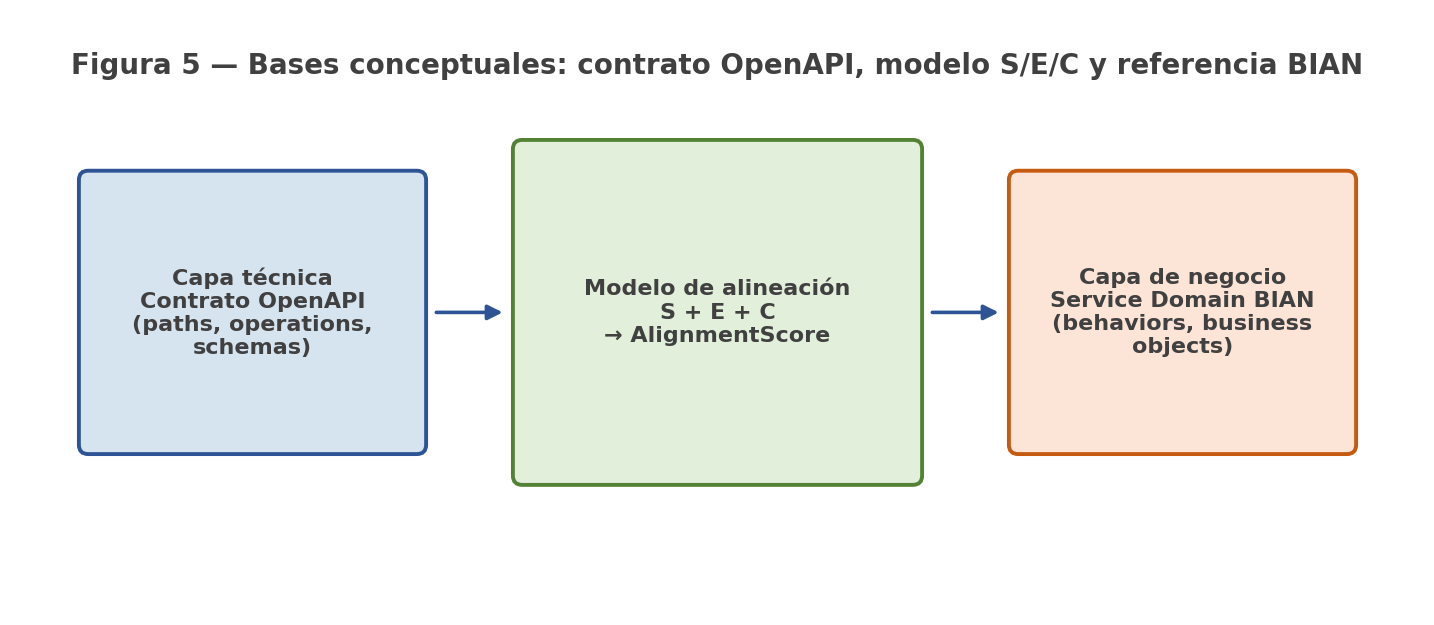
\includegraphics[width=0.92\textwidth]{Figura_05_Bases_Conceptuales}
  \caption{Bases conceptuales: contrato OpenAPI, \ServiceDomain{} BIAN y modelo de alineación S/E/C}
  \label{fig:bases-conceptuales}
\end{figure}
